% Chapter Template

\chapter{Requirements Analysis and Evaluation Strategy} % Main chapter title
\label{Requirements Analysis} % Change X to a consecutive number; for referencing this chapter elsewhere, use \ref{ChapterX}

%----------------------------------------------------------------------------------------
%	SECTION 1
%----------------------------------------------------------------------------------------

This chapter provides an insight into the project requirements followed by demonstrating the project implementation workflow, UI wireframe, data collection, and processing methodology, and concludes with an evaluation strategy.

\section{Requirements Analysis}
This section identifies and outlines the functional and non-functional requirements pertaining to this project. The priority 
of each of these requirements are ranked according to the MSCW prioritization technique. The following color-scheme 
indicates the respective ranking order:

\begin{itemize}
  \item \colorbox{green}{\textbf{Must Have (M)}} - These requirements are fundamental to achieve the aim of this project.
  \item \colorbox{cyan}{\textbf{Should Have (S)}} - These requirements are important to the project but not vital and could be achieved in the long run.
  \item \colorbox{yellow}{\textbf{Could Have (C)}} - These requirements are not fundamental to achieve the aim of this project but would be an added benefit if accomplished.
  \item \colorbox{pink}{\textbf{Want To Have (W)}} - These requirements would be prioritized in later releases of the project.
\end{itemize}

\subsection{Functional and Non-Functional Requirements}
The Functional Requirements (FR's) describes the essential components, purpose, and objectives of this project.
Table \ref{tab:Functional Requirements} tabulates the FR's along with a brief description for the same and its priority according to MSCW prioritization technique. An evaluation 
for each of these functional requirements is specified in section \ref{Evaluation Strategy Section}.

% \subsection{Non-Functional Requirements}
Non-Functional Requirements (NFR's) emphasizes the system's operation which includes its performance, usability, portability, and so on. Table \ref{tab:Non-Functional Requirements} tabulates each of these NFR's and applies the MSCW prioritization technique.

\begin{longtable}{| p{.10\textwidth} | p{.70\textwidth} | p{.10\textwidth} |} 
\hline
\multicolumn{3}{|c|}{\textbf{Functional Requirements}}\\
\hline
\textbf{ID} & \textbf{Description} & \textbf{Priority}  \\
\hline
FR-1 & \textbf{X-ray Segmentation}  & \cellcolor{green}\textbf{M} \\ &  The system shall be able to accept and segment X-ray scans. & \cellcolor{green} \\ \hline 
FR-2 & \textbf{CT Segmentation}  & \cellcolor{cyan}\textbf{S} \\ &  The system shall be able to accept and segment CT scans. & \cellcolor{cyan} \\ \hline 
FR-3 & \textbf{COVID-19 Diagnosis using X-ray Scans}  & \cellcolor{green}\textbf{M} \\ & The system shall be able to classify positive COVID-19 patients from others given test X-ray scans & \cellcolor{green} \\ \hline 
FR-4 & \textbf{COVID-19 Diagnosis using CT Scans}  & \cellcolor{cyan}\textbf{S} \\ &  The system shall be able to classify positive COVID-19 patients from others given test CT scans. & \cellcolor{cyan} \\ \hline
FR-5 & \textbf{Visualize Lung Region of Interest's}  & \cellcolor{green}\textbf{M} \\ &  The system shall be able to interpret and visualize classification results by highlighting lung ROIs. & \cellcolor{green} \\ \hline 
FR-6 & \textbf{Multi-class Diagnosis}  & \cellcolor{pink}\textbf{W} \\ &  The system shall be able to differentiate COVID-19 and Pneumonia (Viral or Bacterial) patients. & \cellcolor{pink} \\ \hline 
FR-7 & \textbf{Web Interface}  & \cellcolor{cyan}\textbf{S} \\ &  The system shall have an interface which presents diagnosis results after segmentation for visualization and analysis purposes. & \cellcolor{cyan} \\ \hline

% \multirowcell{2}{FR2} & 70 COVID-19 & \cellcolor{green} \\ & Others & \multirowcell{-2}{*}{ \cellcolor{green}S}\\ \hline
\caption{Functional Requirements}

  \label{tab:Functional Requirements}
  \end{longtable}

%   \begin{longtable}{| p{.10\textwidth} | p{.70\textwidth} | p{.10\textwidth} |} 
%     \hline
%     \multicolumn{3}{|c|}{\textbf{User Functional Requirements}}\\
%     \hline
%     \textbf{ID} & \textbf{Description} & \textbf{Priority}  \\
%     \hline
%     U-FR-1 & \textbf{Input X-ray Scans}  & \cellcolor{green}\textbf{M} \\ & The user shall be able to provide X-ray scan images as input for COVID-19 diagnosis. & \cellcolor{green} \\ \hline 
%     U-FR-2 & \textbf{Input CT Scans}  & \cellcolor{cyan}\textbf{S} \\ &   The user shall be able to provide CT scan images as input for COVID-19 diagnosis. & \cellcolor{cyan} \\ \hline 
%     U-FR-3 & \textbf{Save Classification Results}  & \cellcolor{green}\textbf{M} \\ & The user shall be able to save and interact with the classification results which highlights the lung ROI's. & \cellcolor{green} \\ \hline 

%     % \multirowcell{2}{FR2} & 70 COVID-19 & \cellcolor{green} \\ & Others & \multirowcell{-2}{*}{ \cellcolor{green}S}\\ \hline
%     \caption{User Functional Requirements}
    
%       \label{tab:User Functional Requirements}
%       \end{longtable}

\vspace{5em}
% \\\\
\begin{longtable}{| p{.10\textwidth} | p{.70\textwidth} | p{.10\textwidth} |} 
  
  \hline
  \multicolumn{3}{|c|}{\textbf{Non-Functional Requirements}}\\
  \hline
  \textbf{ID} & \textbf{Description} & \textbf{Priority}  \\
  \hline
  NFR-1 & \textbf{Environment}  & \cellcolor{yellow}\textbf{C} \\ & The system shall be deployed on a cloud platform such as IBM Cloud. & \cellcolor{yellow} \\ \hline 
  NFR-2 & \textbf{User Interface}  & \cellcolor{cyan}\textbf{S} \\ &   The system shall have an intuitive and user-friendly interface where the user can input scans and receive diagnosis results which could be confirmed by a medical professional. & \cellcolor{cyan} \\ \hline 
  NFR-3 & \textbf{Extensibility}  & \cellcolor{cyan}\textbf{S} \\ & The system shall be flexible to extensions, this includes bug fixes, updated features and performance improvement.& \cellcolor{cyan} \\ \hline 
  NFR-4 & \textbf{Version Control}  & \cellcolor{green}\textbf{M} \\ & All versions of the code shall be published on GitHub which enables version control and be open source.& \cellcolor{green} \\ \hline 
  NFR-5 & \textbf{Documentation}  & \cellcolor{green}\textbf{M} \\ & The code shall include relevant comments and contain an instructions guide to setup the environment and run the code. & \cellcolor{green} \\ \hline 
  NFR-6 & \textbf{Modular Programming}  & \cellcolor{cyan}\textbf{S} \\ & The program functionality shall be separated into independent components to emphasize the scalability of software.& \cellcolor{cyan} \\ \hline 
  NFR-7 & \textbf{Reusability}  & \cellcolor{yellow}\textbf{C} \\ & The code developed shall be reusable by other researches and developers. & \cellcolor{yellow} \\ \hline 

  % \multirowcell{2}{FR2} & 70 COVID-19 & \cellcolor{green} \\ & Others & \multirowcell{-2}{*}{ \cellcolor{green}S}\\ \hline
  \caption{Non-Functional Requirements}
  
    \label{tab:Non-Functional Requirements}
    \end{longtable}


% This chapter provides an insight into the project implementation 
% workflow, UI wireframe, data collection, and processing methodology, 
% and concludes with an evaluation strategy.
\vspace{-2em}
\section{Implementation Workflow}
The activity diagram displayed in Figure \ref{fig:Implementation Methodology} provides a blueprint of the workflow that would be followed for the development phase commencing next semester. 

% The wireframe illustrated in Appendix \ref{Wireframe} displays the expected general layout of the COVID-19 diagnosis portal.

\begin{figure}[H]
 \centering
 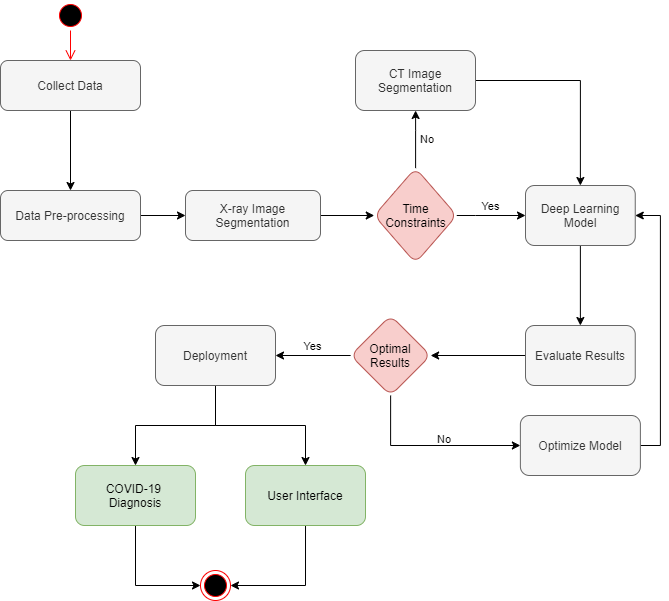
\includegraphics[width=15.5cm, height=11.5cm]{Images/activityDiagram.png}
 \decoRule
 \caption[Implementation Methodology]{Activity Diagram displaying the implementation workflow.}
 \label{fig:Implementation Methodology}
 \end{figure}
 
 \vspace{-2em}
\section{Evaluation Strategy} \label{Evaluation Strategy Section}
Table \ref{tab:Evaluation Strategy} summarizes the methods and strategies used to evaluate each of the Functional Requirements described in Chapter \ref{Requirements Analysis}.

\begin{longtable}{| p{.10\textwidth} | p{.82\textwidth} |} 
\hline
\multicolumn{2}{|c|}{\textbf{Evaluation Strategy}}\\
\hline
\textbf{ID} & \textbf{Description}\\
\hline
FR-1 & \parbox[t]{12.3cm}{\textbf{X-ray Segmentation} \\ The lung segments produced from X-ray scans shall be evaluated based on its capability to identify possible ROIs.}\\\hline
FR-2 & \parbox[t]{12.3cm}{\textbf{CT Segmentation} \\ The lung segments produced from CT scans shall be evaluated based on its capability to identify possible ROIs.}\\\hline
FR-3 & \parbox[t]{12.3cm}{\textbf{COVID-19 Diagnosis using X-ray Scans} \\ The diagnosis results obtained after achieving FR-1 shall be evaluated against various statistical metrics such as Accuracy, Precision and Recall.}\\\hline
FR-4 & \parbox[t]{12.3cm}{\textbf{COVID-19 Diagnosis using CT Scans} \\ The diagnosis results obtained after achieving FR-2 shall be evaluated against various statistical metrics such as Accuracy, Precision and Recall.}\\\hline
FR-5 & \parbox[t]{12.3cm}{\textbf{Visualize Lung Region of Interest's} \\ The ROIs visualized correlates to the observed lung characteristics in COVID-19 patients.} \\\hline
FR-6 & \parbox[t]{12.3cm}{\textbf{Multi-class Diagnosis} \\ The diagnosis results obtained shall be evaluated against various statistical metrics such as Accuracy, Precision and Recall.}\\\hline
FR-7 & \parbox[t]{12.3cm}{\textbf{Web Interface} \\ The user interface developed shall evaluated based on the following metrics, that is, user-friendliness, consistency, familiarity, responsiveness, and intuitiveness\vspace{0.2em}}\\\hline
\caption{Evaluation Strategy}

  \label{tab:Evaluation Strategy}
  \end{longtable}
  
    \vspace{-2em}
\section{Implementation Methodology}
A brief summary of the methodology that would be carried out in semester 2 as well as their evaluation is described in this section.
\subsection{Data Collection}
The two primary sources for collecting open-source anonymized data would be the COVID-19 Kaggle datasets and the scans provided by Cohen et al. \cite{JMD2020} as seen from the literature review. The images obtained shall be separated into X-ray and CT scans separately and furthermore, on the basis of their labels.
\begin{itemize}
    \item \textbf{Testing} - Datasets which correspond to other lung diseases would also be used to analyze the generalizability of the model.
     \item \textbf{Evaluation} - Training would be conducted using  10-fold cross-validation, followed by rigorous verification to prevent the model from either overfitting or underfitting.
\end{itemize}

\subsection{Data Pre-processing}
Before carrying out image segmentation for both X-ray and CT scans, all images in the training dataset shall undergo the same data pre-processing pipeline as per the model's input parameters.
\begin{itemize}
    \item \textbf{Testing} - The model would be tested on images with different dimensions to ensure no input errors are caused.
     \item \textbf{Evaluation} - An input verification technique shall be applied to validate the provided training images before the deep learning workflow commences.
\end{itemize}

\subsection{Image Segmentation}
The provided training images, both X-ray and CT scans shall undergo segmentation such that the ROIs would be highlighted and lead to effective COVID-19 diagnosis
\begin{itemize}
    \item \textbf{Testing} - Multiple image segmentation techniques as suggested by the literature shall be used during the development phase to identify the one that yields the best results.
     \item \textbf{Evaluation} - All models used for experimentation purposes would be documented and the best would be utilized for final demonstration purposes.
\end{itemize}
\subsection{Model Optimization}
As observed in the literature review, multiple studies \cite{CXZ+2020, CYZ+2020, HLR+2020, YHQ+2020, GOM+2020, LLL+2020, CJL+2020, JSB+2020, SFY+2020} indicate variants of the U-Net architecture to be the best suited for CT scan segmentation whereas, for X-rays, variants of ResNet and CNN seem to be ideal as per the research conducted \cite{ZXS+2020, AKP2020, GHT2020, LWA2020}.
\begin{itemize}
    \item \textbf{Testing} - Each of the proposed model variations shall be experimented with for testing purposes, and the results obtained shall be compared to existing literature. 
     \item \textbf{Evaluation} - The results obtained after tweaking the various hyper-parameters for each of the proposed models shall be tracked, thus being able to identify the most optimal set of values.
\end{itemize}


% \section{Research Questions}
% Upon project completion we aim to find answers to the following questions after applying 
% suitable evaluation strategies:

% \begin{itemize}
%   \item Identify whether the ROI's detected by the deep learning model correlates with the lung characteristics observed on COVID-19 patients.
%   \item Compare the results obtained by the deep learning approach with the standard RT-PCR test.
%   \item Feasibility of deploying and utilizing the deep learning model in medical facilities and laboratories for rapid real-time COVID-19 diagnosis.
% \end{itemize}